\subsection{Visitor Pattern}
\label{sec:VisitorDesign}

As can be seen on figure \ref{fig:CompilerProcess}, several steps in the compilation process acts on the AST, with semantic analysis containing both a type checker and a borrow checker evaluating the AST, and the code generator running through the AST to generate the intermediate representation.\\
As the Compiler has to traverse the tree several times, it would be desirable to have a unified way of traversing the structure for all the different steps. The immediate and naive solution would be to implement the different algorithms into the tree nodes directly. This approach has the appeal of making it easy to add new nodes. It does, however, make it difficult to add additional functionality to the compiler, as every addition requires a modification of every node class. It also requires that the nodes transmit information between each other, causing high coupling. A better solution would be to use the visitor design pattern.

The visitor pattern separates algorithms from an object structure by implementing a 'visitor' class which can traverse the tree and perform the correct operations on each node. This allows for additional functionality to be added, without modifying the existing tree (thus following the open-closed principle). As long as every node implements an 'accept' function, new visitors can be added without the need for altering the expression classes at all. A modification of the AST is necessarily more involved when using a visitor, compared to the naive approach, as every visitor must be updated to handle the new type of node, but the structure makes it easy to see where the changes should be made. 

\begin{figure}[h]
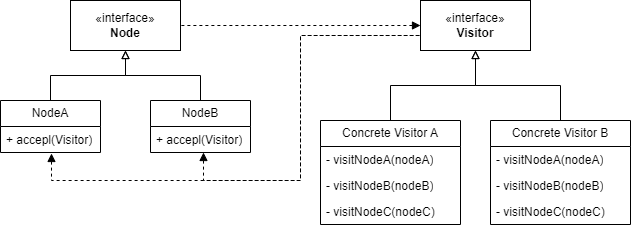
\includegraphics[width=\textwidth]{02-Body/Images/VisitorClassDiag.png}
\caption{Class diagram for Visitor Pattern}
\label{fig:VisitorClassDiagram}
\end{figure}

Figure \ref{fig:VisitorClassDiagram} shows a class diagram for a visitor design. The nodes of the tree all inherit an accept function from the Node interface, which takes a visitor interface as a parameter. The sole purpose of this accept funtcion is to call the correct visit function in the given visitor (nodeA calling visitNodeA(...) etc.). The Concrete visitors inherit Visit functions (visitNodeA(...), visitNodeB(...) etc.) from the Visitor interface, with each visit function taking the corresponding node type as a parameter. The actual functionality is the implemented in the visit functions, and because they have been given the actual node as a parameter, all relevant information is readily available.